%%%%%%%%%%%%%%%%%%%%%%%
% Comp 170, Fall 2019
% Homework 1
% Author: Vladimir Hugec
%%%%%%%%%%%%%%%%%%%%%%%

% This portion of the LaTeX document are configuration 
% You can see it as all the #includes in C++
\documentclass[12pt]{article}

\usepackage{epsfig}
\usepackage{amsmath}
\usepackage{amsthm}
\usepackage{listings}
\usepackage{graphicx}
\usepackage{tikz}

\newtheorem{lemma}{Lemma}
\newtheorem{theorem}{Theorem}

\usepackage{titlesec}
\titleformat{\section}
{\normalfont\Large\bfseries}{Question~\thesection:}{1em}{}

\newlength{\toppush}
\setlength{\toppush}{2\headheight}
\addtolength{\toppush}{\headsep}

\def\subjnum{Comp 170}
\def\subjname{Computation Theory}

\def\doheading#1#2#3{\vfill\eject\vspace*{-\toppush}%
  \vbox{\hbox to\textwidth{{\bf} \subjnum: \subjname \hfil Vladimir Hugec}%
    \hbox to\textwidth{{\bf} Tufts University, Fall 2019 \hfil#3\strut}%
    \hrule}}


\newcommand{\htitle}[1]{\vspace*{1.25ex plus 1ex minus 0ex}%
\begin{center}
{\large\bf #1}
\end{center}} 


%%%%%%%%%%%%%%%%%%%%%%%%%%%%%%%%%%%%%%%%%%%%%%%%%%%%%%%%%%%%%%%%%%%
% BEGIN DOCUMENT
%%%%%%%%%%%%%%%%%%%%%%%%%%%%%%%%%%%%%%%%%%%%%%%%%%%%%%%%%%%%%%%%%%%
\begin{document}
\doheading{2}{title}{Homework 1}

\section{} 
\begin{center}
$L_{1} = \{w | w $ does not contain the substring $000\}$
\end{center}

\subsection{Construct a DFA}

\begin{center}
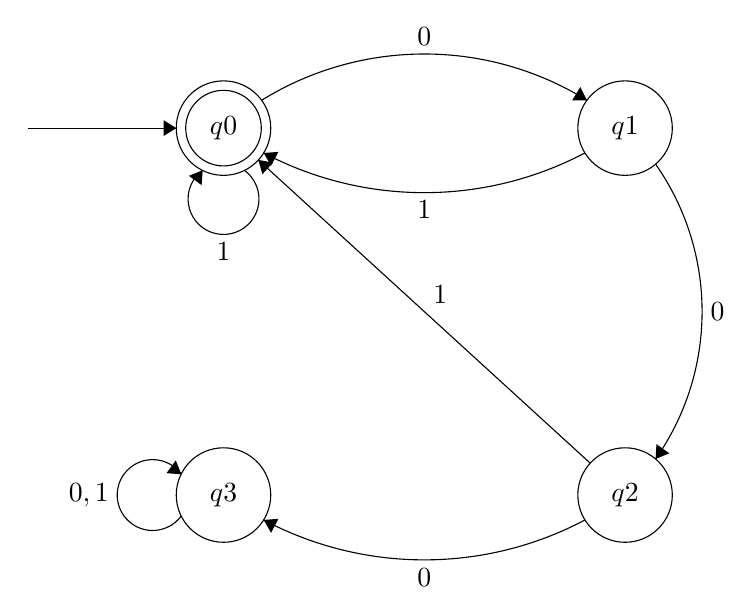
\begin{tikzpicture}[scale=0.2]
\tikzstyle{every node}+=[inner sep=0pt]
\draw [black] (22.6,-19) circle (3);
\draw (22.6,-19) node {$q0$};
\draw [black] (22.6,-19) circle (2.4);
\draw [black] (48.1,-19) circle (3);
\draw (48.1,-19) node {$q1$};
\draw [black] (48.1,-42.3) circle (3);
\draw (48.1,-42.3) node {$q2$};
\draw [black] (22.6,-42.3) circle (3);
\draw (22.6,-42.3) node {$q3$};
\draw [black] (10.2,-19) -- (19.6,-19);
\fill [black] (19.6,-19) -- (18.8,-18.5) -- (18.8,-19.5);
\draw [black] (25.02,-17.232) arc (121.76061:58.23939:19.624);
\fill [black] (45.68,-17.23) -- (45.26,-16.39) -- (44.74,-17.24);
\draw (35.35,-13.79) node [above] {$0$};
\draw [black] (50.037,-21.286) arc (35.01018:-35.01018:16.322);
\fill [black] (50.04,-40.01) -- (50.91,-39.65) -- (50.09,-39.07);
\draw (53.49,-30.65) node [right] {$0$};
\draw [black] (45.554,-43.882) arc (-62.08789:-117.91211:21.798);
\fill [black] (25.15,-43.88) -- (25.62,-44.7) -- (26.09,-43.81);
\draw (35.35,-46.92) node [below] {$0$};
\draw [black] (19.92,-43.623) arc (324:36:2.25);
\draw (15.35,-42.3) node [left] {$0,1$};
\fill [black] (19.92,-40.98) -- (19.57,-40.1) -- (18.98,-40.91);
\draw [black] (23.923,-21.68) arc (54:-234:2.25);
\draw (22.6,-26.25) node [below] {$1$};
\fill [black] (21.28,-21.68) -- (20.4,-22.03) -- (21.21,-22.62);
\draw [black] (45.55,-20.576) arc (-62.20778:-117.79222:21.876);
\fill [black] (25.15,-20.58) -- (25.62,-21.39) -- (26.09,-20.51);
\draw (35.35,-23.6) node [below] {$1$};
\draw [black] (45.89,-40.28) -- (24.81,-21.02);
\fill [black] (24.81,-21.02) -- (25.07,-21.93) -- (25.74,-21.19);
\draw (36.36,-30.16) node [above] {$1$};
\end{tikzpicture}
\end{center}

\subsection{Full Formal Specifications of the Machine}

$ \indent Q = \{q_{0},q_{1},q_{2},q_{3}\}$

$ \Sigma = \{0,1\}$

$ \delta : Q$ x $\Sigma \rightarrow Q $

$ \indent  \delta(q_{0},1) = q_{0}$

$\indent   \delta(q_{0},0) = q_{1}$

$\indent   \delta(q_{1},1) = q_{0}$

$\indent   \delta(q_{1},0) = q_{2}$

$\indent   \delta(q_{2},1) = q_{0}$

$\indent   \delta(q_{2},0) = q_{3}$

$\indent   \delta(q_{3},0) = q_{3}$

$\indent   \delta(q_{3},1) = q_{3}$

$q_{0} \in Q$ is initial state

$ F = q_{0} $

\pagebreak

\section{}

\begin{center}
$L_{2} = \{w | $   $|w| \geq 2$, but w contains less than two 1’s\}
\end{center}

\subsection{DFA for $L_{2} = \{w | $   $|w| \geq 2 \}$ }

\begin{center}
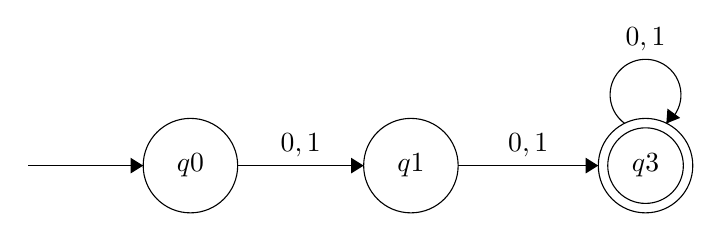
\begin{tikzpicture}[scale=0.2]
\tikzstyle{every node}+=[inner sep=0pt]
\draw [black] (22.9,-20.6) circle (3);
\draw (22.9,-20.6) node {$q0$};
\draw [black] (36.9,-20.6) circle (3);
\draw (36.9,-20.6) node {$q1$};
\draw [black] (51.8,-20.6) circle (3);
\draw (51.8,-20.6) node {$q3$};
\draw [black] (51.8,-20.6) circle (2.4);
\draw [black] (12.6,-20.6) -- (19.9,-20.6);
\fill [black] (19.9,-20.6) -- (19.1,-20.1) -- (19.1,-21.1);
\draw [black] (25.9,-20.6) -- (33.9,-20.6);
\fill [black] (33.9,-20.6) -- (33.1,-20.1) -- (33.1,-21.1);
\draw (29.9,-20.1) node [above] {$0,1$};
\draw [black] (39.9,-20.6) -- (48.8,-20.6);
\fill [black] (48.8,-20.6) -- (48,-20.1) -- (48,-21.1);
\draw (44.35,-20.1) node [above] {$0,1$};
\draw [black] (50.477,-17.92) arc (234:-54:2.25);
\draw (51.8,-13.35) node [above] {$0,1$};
\fill [black] (53.12,-17.92) -- (54,-17.57) -- (53.19,-16.98);
\end{tikzpicture}
\end{center}

\subsection{DFA for  $L_{2} = \{w | $  w contains less than two 1's$\}$}




\begin{center}
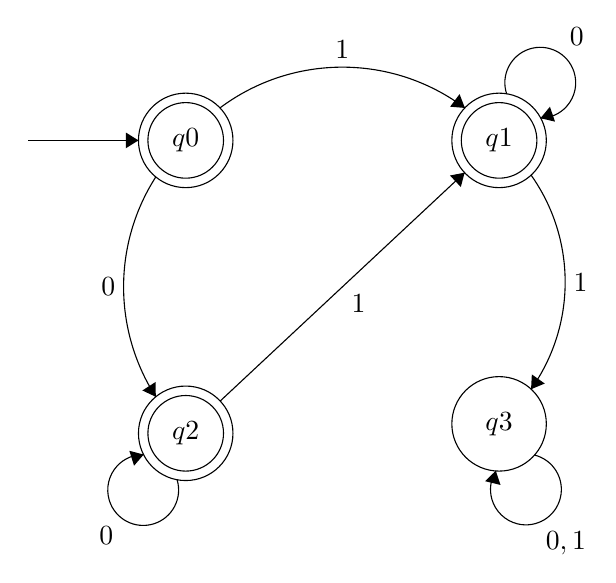
\begin{tikzpicture}[scale=0.2]
\tikzstyle{every node}+=[inner sep=0pt]
\draw [black] (19.5,-24) circle (3);
\draw (19.5,-24) node {$q0$};
\draw [black] (19.5,-24) circle (2.4);
\draw [black] (39.4,-24) circle (3);
\draw (39.4,-24) node {$q1$};
\draw [black] (39.4,-24) circle (2.4);
\draw [black] (19.5,-42.6) circle (3);
\draw (19.5,-42.6) node {$q2$};
\draw [black] (19.5,-42.6) circle (2.4);
\draw [black] (39.4,-42) circle (3);
\draw (39.4,-42) node {$q3$};
\draw [black] (9.5,-24) -- (16.5,-24);
\fill [black] (16.5,-24) -- (15.7,-23.5) -- (15.7,-24.5);
\draw [black] (21.672,-21.94) arc (126.85458:53.14542:12.968);
\fill [black] (37.23,-21.94) -- (36.89,-21.06) -- (36.29,-21.86);
\draw (29.45,-18.85) node [above] {$1$};
\draw [black] (17.603,-40.285) arc (-147.31781:-212.68219:12.935);
\fill [black] (17.6,-40.28) -- (17.59,-39.34) -- (16.75,-39.88);
\draw (15.06,-33.3) node [left] {$0$};
\draw [black] (21.69,-40.55) -- (37.21,-26.05);
\fill [black] (37.21,-26.05) -- (36.28,-26.23) -- (36.97,-26.96);
\draw (30.47,-33.78) node [below] {$1$};
\draw [black] (18.95,-45.537) arc (17.1301:-270.8699:2.25);
\draw (14.45,-48.5) node [below] {$0$};
\fill [black] (16.83,-43.95) -- (15.92,-43.71) -- (16.22,-44.66);
\draw [black] (39.881,-21.051) arc (198.46232:-89.53768:2.25);
\draw (44.33,-18.01) node [above] {$0$};
\fill [black] (42.03,-22.59) -- (42.95,-22.81) -- (42.63,-21.86);
\draw [black] (41.428,-26.2) arc (35.36446:-35.36446:11.75);
\fill [black] (41.43,-39.8) -- (42.3,-39.44) -- (41.48,-38.86);
\draw (44.1,-33) node [right] {$1$};
\draw [black] (41.639,-43.979) arc (76.24902:-211.75098:2.25);
\draw (43.64,-48.78) node [below] {$0,1$};
\fill [black] (39.19,-44.98) -- (38.51,-45.64) -- (39.49,-45.88);
\end{tikzpicture}
\end{center}

\pagebreak

\subsection{DFA for combination of both other DFA's}

\begin{center}
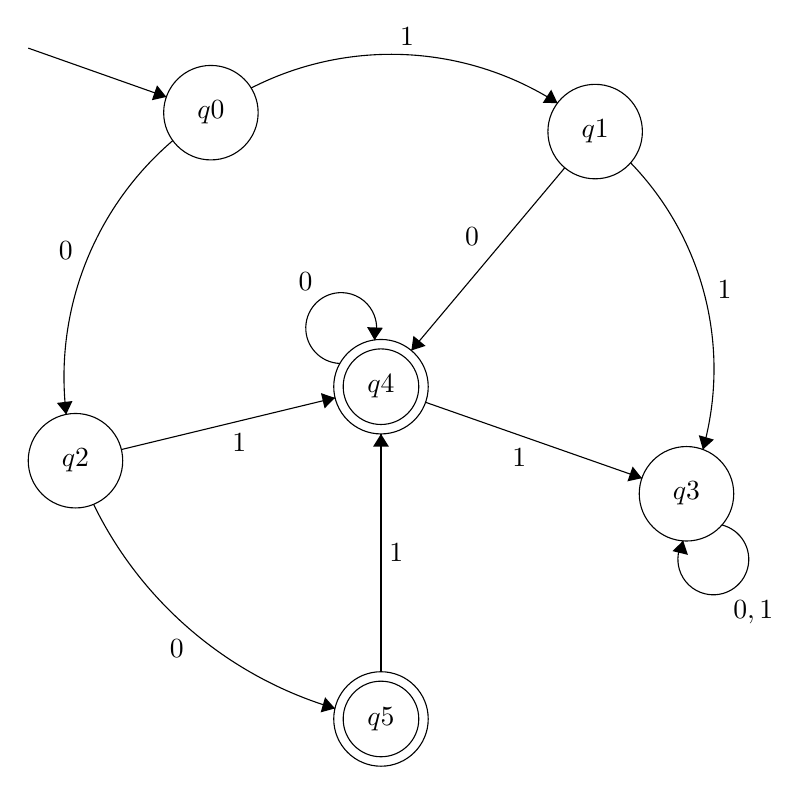
\begin{tikzpicture}[scale=0.2]
\tikzstyle{every node}+=[inner sep=0pt]
\draw [black] (22,-9.1) circle (3);
\draw (22,-9.1) node {$q0$};
\draw [black] (46.4,-10.3) circle (3);
\draw (46.4,-10.3) node {$q1$};
\draw [black] (13.4,-31.2) circle (3);
\draw (13.4,-31.2) node {$q2$};
\draw [black] (52.2,-33.3) circle (3);
\draw (52.2,-33.3) node {$q3$};
\draw [black] (32.8,-26.5) circle (3);
\draw (32.8,-26.5) node {$q4$};
\draw [black] (32.8,-26.5) circle (2.4);
\draw [black] (32.8,-47.6) circle (3);
\draw (32.8,-47.6) node {$q5$};
\draw [black] (32.8,-47.6) circle (2.4);
\draw [black] (10.4,-5) -- (19.17,-8.1);
\fill [black] (19.17,-8.1) -- (18.58,-7.36) -- (18.25,-8.31);
\draw [black] (24.556,-7.535) arc (117.08632:57.28257:19.536);
\fill [black] (44.01,-8.49) -- (43.61,-7.64) -- (43.07,-8.48);
\draw (34.46,-4.87) node [above] {$1$};
\draw [black] (12.814,-28.261) arc (-173.08073:-229.4453:19.756);
\fill [black] (12.81,-28.26) -- (13.21,-27.41) -- (12.22,-27.53);
\draw (13.26,-17.86) node [left] {$0$};
\draw [black] (48.649,-12.281) arc (44.06149:-15.75466:18.831);
\fill [black] (53.24,-30.49) -- (53.94,-29.86) -- (52.98,-29.58);
\draw (54.14,-20.31) node [right] {$1$};
\draw [black] (54.439,-35.279) arc (76.24902:-211.75098:2.25);
\draw (56.44,-40.08) node [below] {$0,1$};
\fill [black] (51.99,-36.28) -- (51.31,-36.94) -- (52.29,-37.18);
\draw [black] (16.32,-30.49) -- (29.88,-27.21);
\fill [black] (29.88,-27.21) -- (28.99,-26.91) -- (29.22,-27.88);
\draw (23.8,-29.42) node [below] {$1$};
\draw [black] (35.63,-27.49) -- (49.37,-32.31);
\fill [black] (49.37,-32.31) -- (48.78,-31.57) -- (48.45,-32.51);
\draw (41.59,-30.43) node [below] {$1$};
\draw [black] (30.201,-25.025) arc (268.14646:-19.85354:2.25);
\draw (28.01,-20.41) node [above] {$0$};
\fill [black] (32.39,-23.54) -- (32.92,-22.76) -- (31.92,-22.72);
\draw [black] (44.47,-12.6) -- (34.73,-24.2);
\fill [black] (34.73,-24.2) -- (35.63,-23.91) -- (34.86,-23.27);
\draw (39.05,-16.96) node [left] {$0$};
\draw [black] (29.878,-46.927) arc (-106.42439:-153.99535:24.884);
\fill [black] (29.88,-46.93) -- (29.25,-46.22) -- (28.97,-47.18);
\draw (19.84,-42.55) node [below] {$0$};
\draw [black] (32.8,-44.6) -- (32.8,-29.5);
\fill [black] (32.8,-29.5) -- (32.3,-30.3) -- (33.3,-30.3);
\draw (33.3,-37.05) node [right] {$1$};
\end{tikzpicture}
\end{center}

\pagebreak

\section{}

Prove that the following language is regular:

\begin{center}
$ L_{3} = \{w | $ if $w$ contains any 0’s, then it contains at least three of them$\}$
\end{center}

\begin{proof}

A language is regular if one can construct a DFA which can recognize it. The following DFA can recognize $L_{3}$ :

\begin{center}
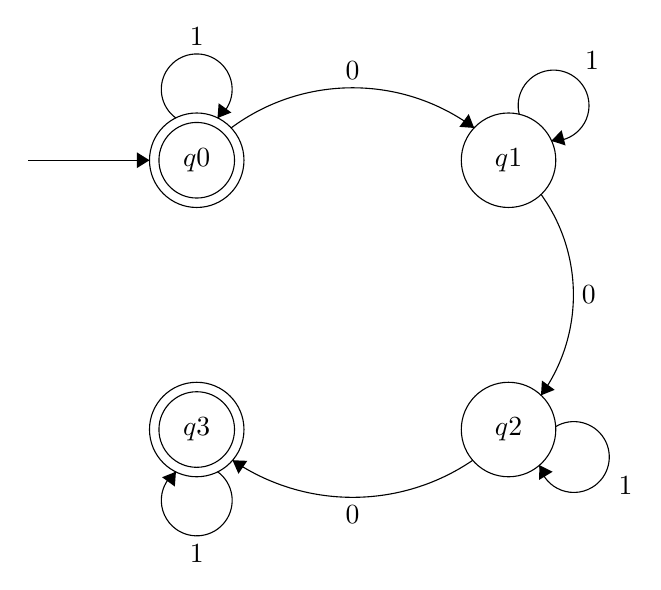
\begin{tikzpicture}[scale=0.2]
\tikzstyle{every node}+=[inner sep=0pt]
\draw [black] (24.2,-23.4) circle (3);
\draw (24.2,-23.4) node {$q0$};
\draw [black] (24.2,-23.4) circle (2.4);
\draw [black] (44,-23.4) circle (3);
\draw (44,-23.4) node {$q1$};
\draw [black] (44,-40.5) circle (3);
\draw (44,-40.5) node {$q2$};
\draw [black] (24.2,-40.5) circle (3);
\draw (24.2,-40.5) node {$q3$};
\draw [black] (24.2,-40.5) circle (2.4);
\draw [black] (13.5,-23.4) -- (21.2,-23.4);
\fill [black] (21.2,-23.4) -- (20.4,-22.9) -- (20.4,-23.9);
\draw [black] (22.877,-20.72) arc (234:-54:2.25);
\draw (24.2,-16.15) node [above] {$1$};
\fill [black] (25.52,-20.72) -- (26.4,-20.37) -- (25.59,-19.78);
\draw [black] (26.382,-21.35) arc (126.57669:53.42331:12.953);
\fill [black] (41.82,-21.35) -- (41.47,-20.47) -- (40.88,-21.28);
\draw (34.1,-18.3) node [above] {$0$};
\draw [black] (46.062,-25.566) arc (35.72675:-35.72675:10.933);
\fill [black] (46.06,-38.33) -- (46.93,-37.98) -- (46.12,-37.39);
\draw (48.62,-31.95) node [right] {$0$};
\draw [black] (44.683,-20.491) arc (194.52754:-93.47246:2.25);
\draw (49.3,-17.7) node [above] {$1$};
\fill [black] (46.72,-22.17) -- (47.62,-22.46) -- (47.37,-21.49);
\draw [black] (46.983,-40.321) arc (121.16635:-166.83365:2.25);
\draw (50.96,-44.06) node [right] {$1$};
\fill [black] (45.96,-42.76) -- (45.94,-43.7) -- (46.8,-43.18);
\draw [black] (41.729,-42.451) arc (-55.68822:-124.31178:13.534);
\fill [black] (26.47,-42.45) -- (26.85,-43.31) -- (27.41,-42.49);
\draw (34.1,-45.31) node [below] {$0$};
\draw [black] (25.523,-43.18) arc (54:-234:2.25);
\draw (24.2,-47.75) node [below] {$1$};
\fill [black] (22.88,-43.18) -- (22,-43.53) -- (22.81,-44.12);
\end{tikzpicture}
\end{center}
\end{proof}

\subsection{Full Formal Specifications of the Machine}

$ \indent Q = \{q_{0},q_{1},q_{2},q_{3}\}$

$ \Sigma = \{0,1\}$

$ \delta : Q$ x $\Sigma \rightarrow Q $

$ \indent  \delta(q_{0},1) = q_{0}$

$\indent   \delta(q_{0},0) = q_{1}$

$\indent   \delta(q_{1},1) = q_{1}$

$\indent   \delta(q_{1},0) = q_{2}$

$\indent   \delta(q_{2},1) = q_{2}$

$\indent   \delta(q_{2},0) = q_{3}$

$\indent   \delta(q_{3},1) = q_{3}$

$q_{0} \in Q$ is initial state

$ F = \{q_{0},q_{3}\} $



\end{document}
%%%%%%%%%%%%%%%%%%%%%%%%%%%%%%%%%%%%%%%%%%%%%%%%%%%%%%%%%%%%%%%%%%%%%%

